


\section{Quadratic programming}

Quad programming text \cite{cameraModule}

\subsection{finding trajectory constrained}
When obstacles are discovered, the problem becomes much more complicated. Some predictions lead to collision. A general equation must be found, what decides which predictions are feasible and which are not. If we want to keep the optimization problem convex, this equation will take form of linear inequalities. 

Unfortunately, the predicted positions must also lie in a convex space. That is important, because 
% need proof
obstacles usually don't take form of convex constraints. For example walls can be considered convex constraints, but for example people, cars and buildings must be avoided by constraining the area in not convex way as shown in figure \ref{fig:avoidance}. Therefore a whole new approach must be applied. 

\begin{figure}[H]
\centering
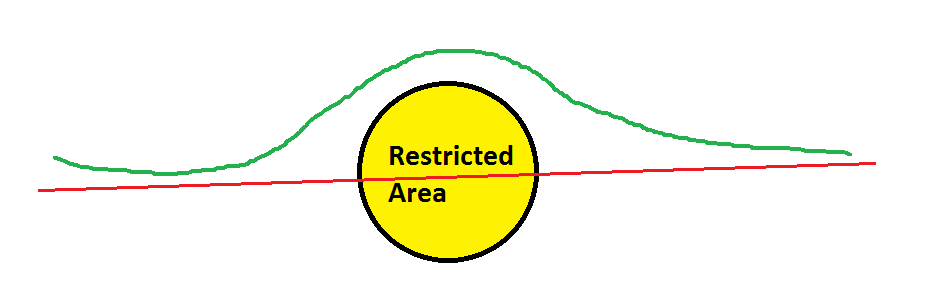
\includegraphics[width=0.7\textwidth]{fig/avoidance.png}
\caption{Not convex avoidance. temporary sketch.}
\label{fig:avoidance}
\end{figure}

For experiment purposes, obstacles will be first approximated with circle and than with half plain. A whole new approach must be applied, because the desired avoidance trajectory might not lie in the allowed space, the great advantage of 


Let's suppose, that the UAV trajectory is a line connecting all predicted positions. If we make sure, that all the positions lie inside the convex space, the whole trajectory has to lie inside a convex space. This is based on the definition of convex space
\begin{equation}
\label{eq:convex_definition}
a,b\in \textbf{M}: \{\lambda a+(1-\lambda) b \mid 0 \leq \lambda \leq 1 \}\in \textbf{M}
\end{equation}
where $\textbf{M}$ is a convex space. 

The linear constrained quadratic programming problem is defined as 


%%  = argmin \frac{1}{2} \textbf{X^T H x} + c^T x

\begin{equation}
\begin{split}
u^\star = arg\ min\ \frac{1}{2} \textbf{u}^T \textbf{Hu}\\
s.\ t. \textbf{A}_c \textbf{u}\leq \textbf{b}_c,\\
\end{split}
\label{eq:quadprog_constrained_definition}
\end{equation}

where $\textbf{A}_c$



